\begin{frame}{Mock Galaxy Catalogues}
    
    Mock galaxy catalogues, artificial galaxy catalogues created using simulations, have many uses in astronomy and cosmology:
    \begin{itemize}
        \item Direct comparison to observations to test theories and assumptions
        \item Estimate statistical and systematic errors
        \item Planning future surveys, what can we expect to find?
        \item Development of analysis tools for observational data
    \end{itemize}
    
\end{frame}

\begin{frame}{Creating Mock Galaxy Catalogues}
    
    There are various approaches on how to obtain mock galaxy catalogues.
    
    Essentially, one can differentiate between two basic approaches:
    
    \begin{itemize}
        \item Physical models
        \item Empirical models
    \end{itemize}
    
\end{frame}


\begin{frame}{Physical Models}
    
    Simulate or parametrise the physics of galaxy formation (e.g. gas cooling, star formation, feedback processes).
    
    Examples: 
    \begin{itemize}
        \item Full hydrodynamical simulation of the Universe
        \item Semi-Analytic models: approximate some processes with analytical prescriptions, constrain parameters of prescriptions with empirical data
    \end{itemize}
    
    Problems:
    \begin{itemize}
        \item Some processes are still not fully understood
        \item Computationally expensive
    \end{itemize}
    
\end{frame}

\begin{frame}{Empirical Models}
    
    Don't try to explain how exactly galaxies form, just to predict where and how many galaxies should be and what properties they should have based on some very simple assumptions.
    
    Key assumption: Galaxies form in condensates (``\emph{haloes}'') of dark matter.
    
    $\Lambda$CDM model states that the Universe is made up from $\sim 5\%$ baryonic (``ordinary'') matter, $\sim 25\%$ dark matter and $\sim 70 \%$ dark energy.
    Over time, the matter in the Universe will clump together and galaxies form in centres of these clumps.
    
\end{frame}


\begin{frame}{DMO Simulations}
    For computational efficiency, neglect baryonic effects in the Universe and replace the baryonic matter with dark matter in order to preserve the total matter content (``\emph{dark matter only}'' simulations).
    
%    Current state-of-the-art: $2\times 10^{12}$ particle simulation \parencite{PKDGRAV}.
    
    With DMO simulations available, a galaxy-halo connection is necessary.
\end{frame}


\begin{frame}{Empirical galaxy-halo connections}
    \begin{itemize}
        \item HOD: gives probability distribution of the number of galaxies that meet some criteria, e.g. minimal mass threshold
        \item Conditional stellar mass/luminosity functions: Specify full distribution of galaxy masses/luminosities for a given halo mass
        \item Abundance Matching: Most massive galaxy lives in most massive halo. Assign galaxies to haloes by rank-order.
    \end{itemize}
    
    The parameters of these techniques are constrained by observational data to reproduce galaxy distributions and properties.
    
\end{frame}


\begin{frame}{SMHM relation}
    
    With these techniques, a stellar-mass-halo-mass-relation can be parametrised and constrained:
    
    \begin{align}
    \log_{10}(M_*(M_h)) &= 
    \log_{10}(\epsilon M_1) + 
    f \left(\log_{10} \left( \frac{M_h}{M_1} \right) \right) - f(0)
    \label{eq:behroozi_SMHM} \\
    %
    f(x) &= -\log_{10}(10^{\alpha x} + 1) + 
    \delta \frac{ [\log_{10}(1+\exp(x))]^\gamma }{1 + \exp(10^{-x})}
    \label{eq:behroozi_fx}
    \end{align}
    
    \parencite{Behroozi}
   
    However, to get accurate galaxy catalogues, some more things need to be considered.
    
\end{frame}




\begin{frame}{Hierarchical Structure Formation}
    In the hierarchical structure formation picture, large haloes are thought to form mainly through consecutive merging events of smaller haloes and accretion of matter too small to be recognised as a halo.
    
    \begin{figure}[H]
        \centering
        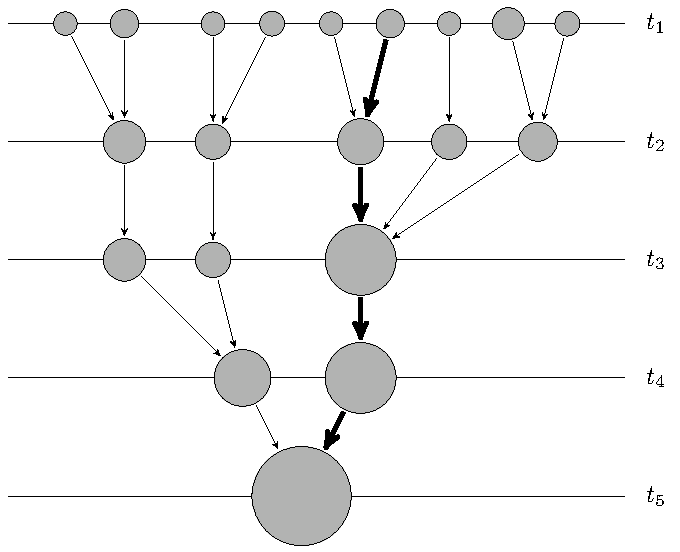
\includegraphics[width=.5\textwidth]{../report/images/tikz/mergertree.pdf}
        \caption{\tiny A merger tree showing the formation history of some halo over cosmic time through a series of merging events with $t_1 < t_2 < t_3 < t_4 < t_5$.}
        \label{fig:mergertree_scheme}
    \end{figure}
    
\end{frame}




\begin{frame}
    
    Due to the hierarchical structure formation, haloes are expected to be spatially nested, i.e. to contain subhaloes.
    
    Over time, the material from subhaloes within a host halo will be stripped due to tidal forces. The tidal stripping affects the outer regions of the subhalo much stronger than regions close to its centre, where it's galaxy is located.
    
    $\Rightarrow$ instead of current mass $M_h$, use peak mass or mass at accretion for subhaloes 
    
    What if subhaloes are stripped of so much mass that they can't be identified as substructure in the host's density field any longer?
    
    $\Rightarrow$ Their galaxy still needs to be kept track of (''\emph{orphan galaxies}'')
    
\end{frame}



{
    \setbeamertemplate{background}
    {\vbox to \paperheight{\vspace{1.2cm}\hbox to \paperwidth{\hfil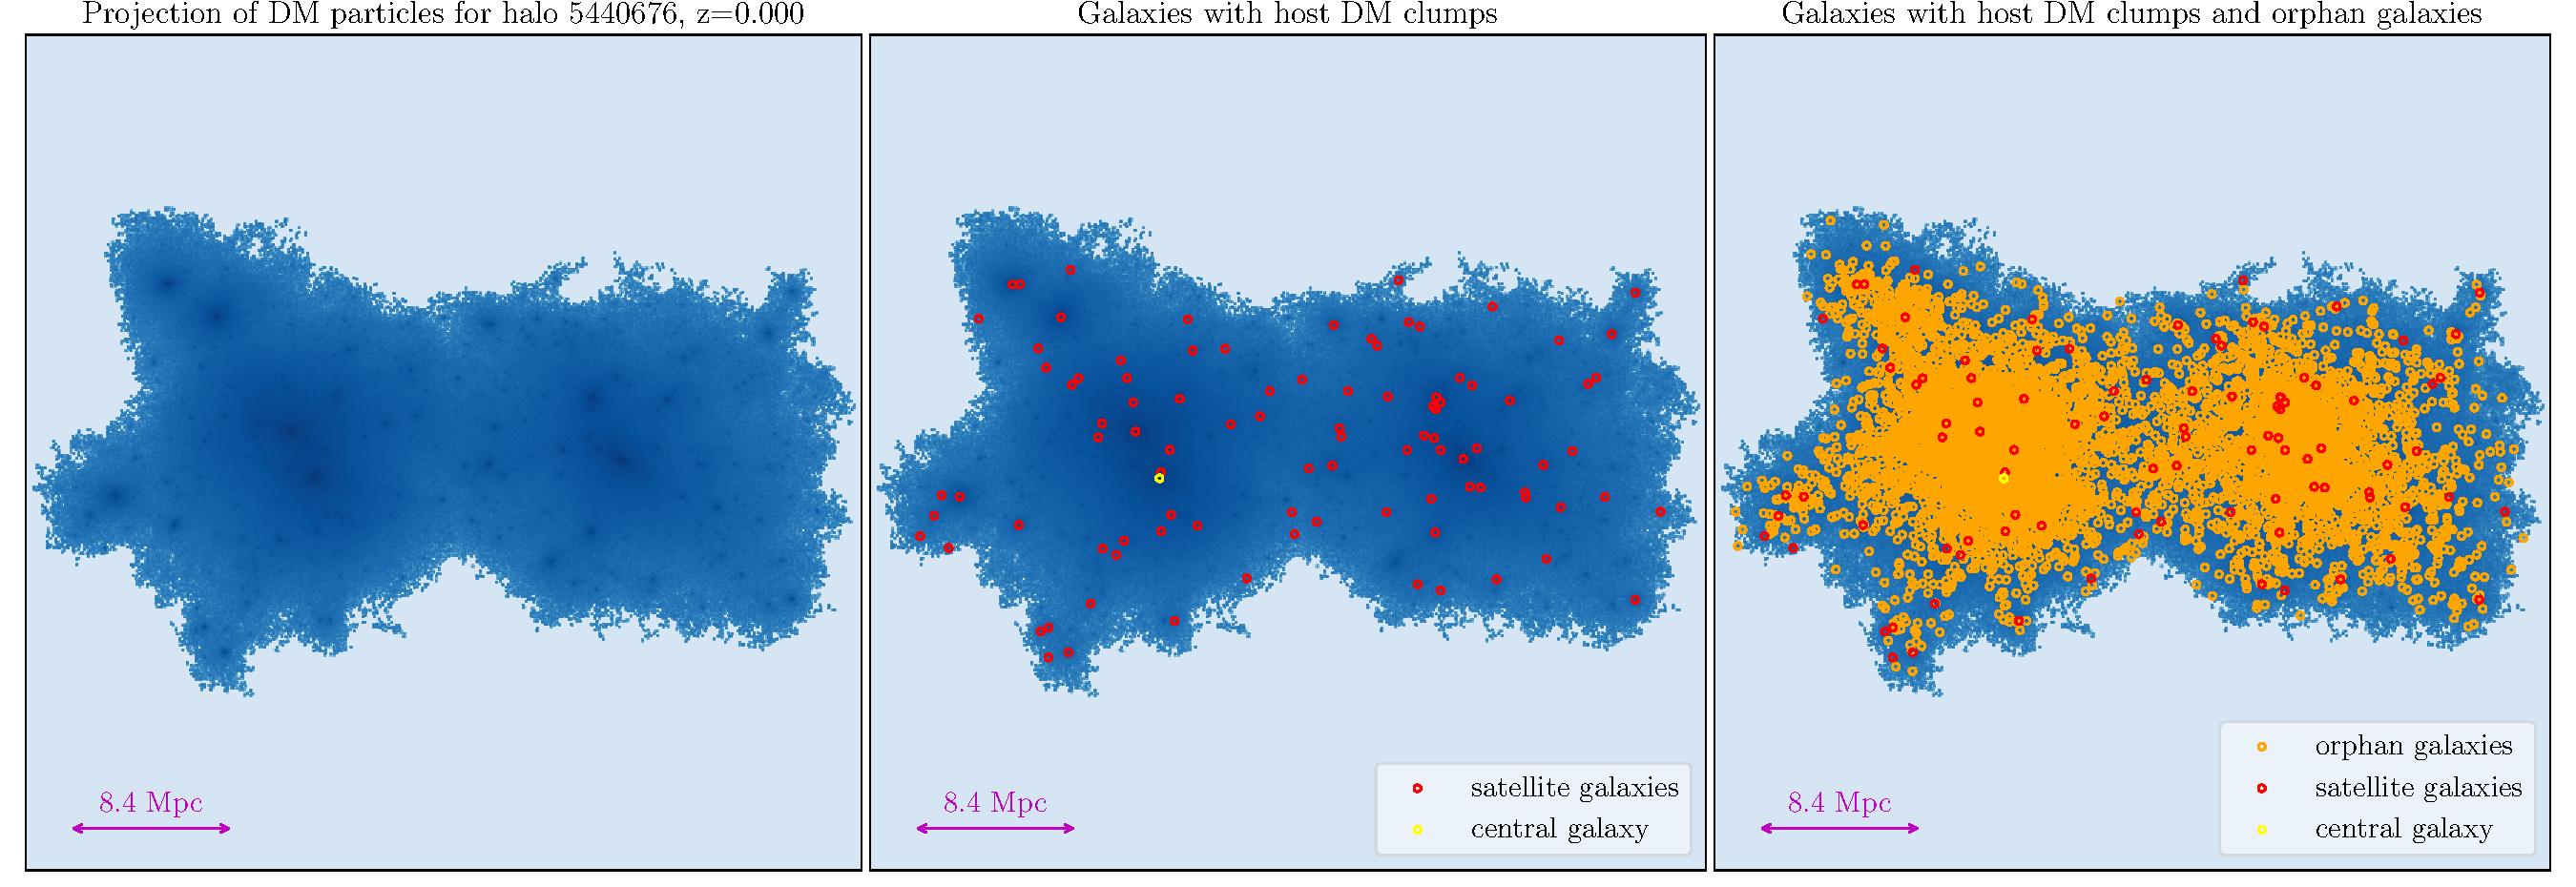
\includegraphics[width=\paperwidth]{../report/images/galaxies/100MPC/halostats_image_output_00041-halo-5440676.pdf}\hfil}\vfil}}
    \begin{frame}
        \frametitle{Orphans and Merger Trees}
        \vspace{4.5cm}
%        {\center \footnotesize \setstretch{0.2}  

        {\setstretch{0.5}
            \small
            \texttt{Projection along the $z$-axis of the most massive halo from a $512^3$ particle simulation, with positions of galaxies at $z=0$ shown
                } \\[.5em]
        }
        
        For accurate mock galaxy catalogues, the formation history of dark matter haloes is necessary.
        
        $\Rightarrow$ need ``\emph{merger trees}'', which show that formation history
    \end{frame}
}

\begin{frame}{Goals of This Thesis}
    \begin{itemize}
        \item Implement an algorithm into \textsc{ramses} \parencite{ramses} to create mock galaxy catalogues from dark matter simulations on the fly and in parallel.
        
        \item For mock galaxy catalogues, first dark matter halo merger trees must be obtained, also on the fly and in parallel.
    \end{itemize}
\end{frame}
